% c11 —— §5 KP 方程理论概要；§5.1–§5.3（原书 p.76–83，末段延伸至 p.84 页首收尾）
% 负责：trans-f

% ===== 原书 p.76 =====
\section{KP 方程理论概要}

本节讲述 KP 方程理论的概要，但主要内容是佐藤方程以及用 Schur 函数展开 $\tau$ 函数。叙述按以下顺序进行。（更详细的文献举 [Sa]。）

\begin{enumerate}[label=\arabic*.,leftmargin=2.4em,itemsep=5pt,topsep=5pt]
\item 构造一个线性微分方程 $Wf=0$，使给定的 $d$ 维有限维函数空间 $V$ 为其解空间。这里 $W$ 是 rank 为 $d$ 的线性微分算子。$\dim=d$ 的向量空间 $V$ 的全体，与 rank 为 $d$ 的微分算子大致成 $1:1$ 对应。（若限制在 Wronskian 处处不为零的范围内，则是 $1:1$。）

\item 在 $\C[x]$ 内 $\dim=d$ 的向量空间全体所成的 Grassmann variety $Grass(d)$ 中，考虑一个特殊的流。它由与 $\partial=\frac{d}{dx}$ 可交换的线性算子中的幂零元素全体 $Z_n(\partial)$ 作为单参数子群生成。$Z_n(\partial)=\partial\C[[\partial]]$，这在拓扑上由 $\partial,\partial^2,\dots$ 生成。也就是由
\[
\{\exp(z)\in\Aut(Grass(d))\mid z\in Z_n(\partial)\}
\]
定出的流。设 $V\in Grass(d)$，把与 $\exp(z)V$ 对应的 rank $d$ 微分算子记作 $W(z,V)$。此时该微分算子的系数，经由 $V$ 的 Pluecker 坐标与 $z=t_1\partial+t_2\partial^2+\cdots$ 的坐标 $(t_1,t_2,\dots)$ 表示出来。也就是说，它由作为 Pluecker 坐标的母函数的 $\tau$ 函数表示。

\item 在 $Z_n(\partial)$ 上以 $z=t_1\partial+\cdots+t_N\partial^N$ 引入坐标 $t=(t_1,t_2,\dots,t_N)$，再考虑关于 $W=W(t,V)$ 的微分方程 $(S_d)$。这是以 $W$ 的系数为未知函数、关于 $t_i$ 的非线性偏微分方程。由此比较 2.\ 与 3.\ 可知：3.\ 的这个非线性偏微分方程具有由 $Grass(d)$ 参数化的解，且该解可写成 $\tau$ 函数。$(S_d)$ 是
\[
W=\partial^d+a_1\partial^{d-1}+\cdots+a_d
\]
的系数 $a_1,\dots,a_d$ 为未知函数、以 $t_1,\dots,t_N$ 为变量的偏微分方程。而对 $(S_d)$ 的解 $W$，$W\partial$ 是 $(S_{d+1})$ 的一种特殊形式的解。这样考虑 $(S_d)$ 关于 $d$ 的相容性时，若要同时处理所有的 $d$，自然的做法是推广为拟微分算子
\[
W=1+a_1\partial^{-1}+a_2\partial^{-2}+\cdots
\]
% ===== 原书 p.77 =====
的系数 $a_1,a_2,\dots$ 为未知函数的微分方程。在这一范畴中考虑，$(S_d)$ 便是 $a_{d+1}=a_{d+2}=\cdots=0$ 的解。一般地，要构造取值于 $1+\partial^{-1}\C[[\partial^{-1}]]$、无法在有限处截断的解，本质上必须构造不是 $Grass(d)$ 的并的 Grassmann variety。

\item 配合 Kontsevich 论文中的情形，作可以想到的那种电荷共轭变换，来表示 $\tau$ 函数。把 $\C[[x]]$ 看作 $\C[\partial]$-module 时，它同构于 $\C((\partial^{-1}))/\C[\partial]$。把 $\partial^{-1}$ 的记号改写为 $\xi$，把 $\C((\xi))/\C[\xi^{-1}]$ 看作 $\C[\partial]$-module。此时，对 $\C((\xi))$ 中满足适当条件的函数列 $f_1,f_2,\dots$ 写出 $\tau$ 函数。这时 $\tau$ 函数可用行列式写出。

\item 最后在本章末尾，用 Harish-Chandra 定理证明：具有矩阵积分表示的函数确实为 KP 方程的 $\tau$ 函数。
\end{enumerate}

\transnote{原书对本名的拼写不统一：§5.1 与 §5.3 的标题（原书 p.77、p.81）均作 GRASMANN，正文 p.76 作 Grassman、p.77 作 Grasmman、p.83 作 Gasmman；此外把 Plücker 一律拼作 Pluecker，把 nilpotent 拼作 niponent。译本统一写作 Grassmann variety 与 Pluecker 坐标；Pluecker 坐标即通行的 Plücker 坐标。}

\transnote{原书此处作「荷電共役変換」，而 §0（原书 p.2）作「共役荷電変換」，二者同指电荷共轭变换。}

\subsection{Grassmann variety 与微分算子的对应}

设 $V$ 为 $\C$ 上可微函数的 $d$ 维子空间，$f_1,\dots,f_d$ 为 $V$ 的基；再设 $g$ 含于 $V$，则
\[
(*)\qquad
\det
\begin{pmatrix}
f_1 & \partial f_1 & \cdots & \partial^d f_1\\
f_2 & \partial f_2 & \cdots & \partial^d f_2\\
 & \cdots & \cdots & \\
f_d & \partial f_d & \cdots & \partial^d f_d\\
g & \partial g & \cdots & \partial^d g
\end{pmatrix}
\]
若 Wronskian
\[
W(f_1,\dots,f_d)=\det
\begin{pmatrix}
f_1 & \partial f_1 & \cdots & \partial^{d-1}f_1\\
\vdots & & & \vdots\\
f_d & \partial f_d & \cdots & \partial^{d-1}f_d
\end{pmatrix}
\]
不为 $0$，则把它看作关于 $g$ 的微分方程，即为 $d$ 阶线性微分方程，故其解与由 $f_1,\dots,f_d$ 张成的 $V$ 一致。把 $(*)$ 作余子式展开，得到
\[
\bigl[W(f_1,\dots,f_d)\partial^d+(\partial W(f_1,\dots,f_d))\partial^{d-1}+\cdots\bigr]g=0
\]

% ===== 原书 p.78 =====
于是除以 $W(f_1,\dots,f_d)$，得到 monic 微分方程
\[
\begin{gathered}
W=\frac{W(f_1,\dots,f_d)\partial^d+(\partial W(f_1,\dots,f_d))\partial^{d-1}+\cdots}{W(f_1,\dots,f_d)}\\
Wg=0
\end{gathered}
\]
此时 $W$ 只依赖于 $d$ 维子空间，故写作 $W=W(V,\partial)$。反之，rank $d$ 的线性微分算子有 $d$ 个独立解，由此可构成 $V$。在这个意义上，Wronskian 处处不为零的 $d$ 维向量空间 $V$ 与 $d$ 阶 monic 线性微分算子成 $1:1$ 对应。

\subsection{Grassmann variety 上的动力系统与 $\tau$ 函数的展开}

特别考虑含于 $\C[x]$ 的 $d$ 维子空间。这样的子空间全体记作 $Grass(d)$。$\C[x]$ 带有关于次数的滤过。保持该滤过且与 $\partial$ 交换的幂零线性映射全体，可等同于 $Z_n(\partial)=\partial\C[[\partial]]$。考虑前述的流 $\exp(z)$（$z\in Z_n(\partial)$），对 $V\in Grass(d)$，把与 $\exp(z)V\in Grass(d)$ 对应的微分算子记作 $W(z,V)$。写作 $z=t_1\partial+t_2\partial^2+\cdots$，把它看作 $t_1,t_2,\dots$ 的函数，记作 $(t,V)$。下面计算 $W(t,V)$。设 $V$ 的基为 $f_i=\sum_{j=0}^N a_{ij}x^j/j!$（$i=1,\dots,d$），令 $f_i(x,t)=\exp(z)f_i(x)$，则 $\exp(z)V$ 由 $f_1(x,t),\dots,f_d(x,t)$ 生成。试计算其 Wronskian 矩阵 $W(f_1(x,t),\dots,f_d(x,t))$。取 $1,x,x^2/2,\dots,x^N/N!$ 作为 $\C\oplus\C x\oplus\cdots\oplus\C x^N$ 的基，把 $f_1,\dots,f_d$ 与列向量 ${}^{t}(a_{i0},\dots,a_{iN})$ 等同起来。此时若用矩阵表示 $\partial$，则为
\[
\Lambda=
\begin{pmatrix}
0 & 1 & 0 & \cdots & 0\\
 & & \cdots & & \\
0 & 0 & \cdots & 0 & 1\\
0 & 0 & \cdots & 0 & 0
\end{pmatrix}
\]

% ===== 原书 p.79 =====
可写成如此。又，
\[
\begin{aligned}
\exp(x\Lambda)
\begin{pmatrix}
a_{i0}\\ \vdots\\ a_{iN}
\end{pmatrix}
&=
\begin{pmatrix}
1 & x & \frac{x^2}{2} & \cdots\\
0 & 1 & x & \cdots\\
 & & \cdots & \\
0 & 0 & \cdots & 0
\end{pmatrix}
\begin{pmatrix}
a_{i0}\\ \vdots\\ a_{iN}
\end{pmatrix}\\
&=
\begin{pmatrix}
f_i\\ \vdots\\ \partial^N f_i
\end{pmatrix}
\end{aligned}
\]
可写成如此。由此，
\[
\begin{aligned}
&\exp(t_1\Lambda+\cdots+t_N\Lambda^N)
\begin{pmatrix}
f_1 & f_2 & \cdots & f_d\\
\partial f_1 & \partial f_2 & \cdots & \partial f_d\\
 & \cdots & \cdots & \\
\partial^N f_1 & \partial^N f_2 & \cdots & \partial^N f_d
\end{pmatrix}\\
&\qquad=\exp\bigl((x+t_1)\Lambda+t_2\Lambda^2+\cdots+t_N\Lambda^N\bigr)
\begin{pmatrix}
a_{10} & \cdots & a_{d0}\\
 & \cdots & \\
a_{1N} & \cdots & a_{dN}
\end{pmatrix}\\
&\qquad=\exp\bigl((x+t_1)\Lambda+t_2\Lambda^2+\cdots+t_N\Lambda^N\bigr)\xi
\end{aligned}
\]
可以写成如此。这里 $\xi$ 是 $V$ 的 frame。
\[
\xi=
\begin{pmatrix}
a_{10} & \cdots & a_{d0}\\
 & \cdots & \\
a_{1N} & \cdots & a_{dN}
\end{pmatrix}
\]
由于 $x$ 必定以 $x+t_1$ 的形式出现，故在 $x=0$ 时求出即可。此时 Wronskian determinant 为
\[
\det
\begin{pmatrix}
f_1 & f_2 & \cdots & f_d\\
\partial f_1 & \partial f_2 & \cdots & \partial f_d\\
 & \cdots & \cdots & \\
\partial^{d-1}f_1 & \partial^{d-1}f_2 & \cdots & \partial^{d-1}f_d
\end{pmatrix}
=\det\bigl((I_d,0)\exp(t_1\Lambda+\cdots+t_N\Lambda^N)\xi\bigr)
\]

\transnote{原书把 $\exp(x\Lambda)$ 的最后一个行向量印作 $(0,0,\cdots,0)$；按 $\Lambda$ 的幂零 Jordan 块形状，该行末项应为 $1$。译文照原文排印。}

% ===== 原书 p.80 =====
成为如此。现引入新变量 $t_i=\frac{1}{i}\sum_{j=1}^N\lambda_j^i$，则
\[
\begin{aligned}
\exp(t_1\Lambda+\cdots+t_N\Lambda^N)
&=\prod_{i=1}^N\exp\Bigl(\lambda_i\Lambda+\frac{1}{2}\lambda_i^2\Lambda^2+\cdots+\frac{1}{N}\lambda_i^N\Lambda^N\Bigr)\\
&=\prod_{i=1}^N(1-\lambda_i\Lambda)^{-1}\\
&=\sum_{i=0}^N m_i(\lambda)\Lambda^i\\
&=
\begin{pmatrix}
1 & m_1 & m_2 & \cdots & m_N\\
0 & 1 & m_1 & \cdots & m_{N-1}\\
 & & \cdots & &
\end{pmatrix}
\end{aligned}
\]
这里 $m_i$ 是称作 complete monomial 的对称函数。对 $0\le i_1<i_2<\cdots<i_d$，用 Jacobi–Trudi 等式
\[
\det
\begin{pmatrix}
m_{i_1} & \cdots & m_{i_d}\\
m_{i_1-1} & \cdots & m_{i_d-1}\\
 & \cdots & \\
m_{i_1-d+1} & \cdots & m_{i_d-d+1}
\end{pmatrix}
=S_Y(\lambda_1,\dots,\lambda_N)
\]
变形 Wronskian。这里 $Y$ 是 Young tableau $Y=(i_d,i_{d-1},\dots,i_1)-(d-1,d-2,\dots,0)$，$S_Y$ 是关于 $\lambda_1,\dots,\lambda_N$ 的 Schur 对称函数。
\[
S_Y(t)=\frac{\det
\begin{pmatrix}
\lambda_1^{i_1} & \cdots & \lambda_1^{i_d}\\
\vdots & & \vdots\\
\lambda_m^{i_1} & \cdots & \lambda_m^{i_d}
\end{pmatrix}}{\prod_{i<j}(\lambda_i-\lambda_j)}
\]

\transnote{原书此处 $S_Y(t)$ 的分子末行为 $\lambda_m^{i_1},\dots,\lambda_m^{i_d}$，分母作 $\prod_{i<j}(\lambda_i-\lambda_j)$；而 $S_Y$ 通篇只用到 $\lambda_1,\dots,\lambda_N$，$m$ 未给出定义，疑为 $N$（或 $d$）之误。译文照原文排印。}
把 $S_Y$ 看作 $t=(t_1,\dots,t_N)$ 的函数时，写作 $S_Y(t)$。对 Young diagram $Y$，把 Pluecker 坐标 $\xi_Y$ 定义为
\[
\xi_Y=\det
\begin{pmatrix}
a_{1i_1} & \cdots & a_{di_1}\\
 & \cdots & \\
a_{1i_d} & \cdots & a_{di_d}
\end{pmatrix}
\]
则
\[
W(f_1(0,t),\dots,f_d(0,t))=\sum_Y S_Y(t)\xi_Y
\]

% ===== 原书 p.81 =====
可以写成如此。这里 $Y$ 跑遍纵横尺寸落在下图范围内的 Young tableau。
\begin{center}
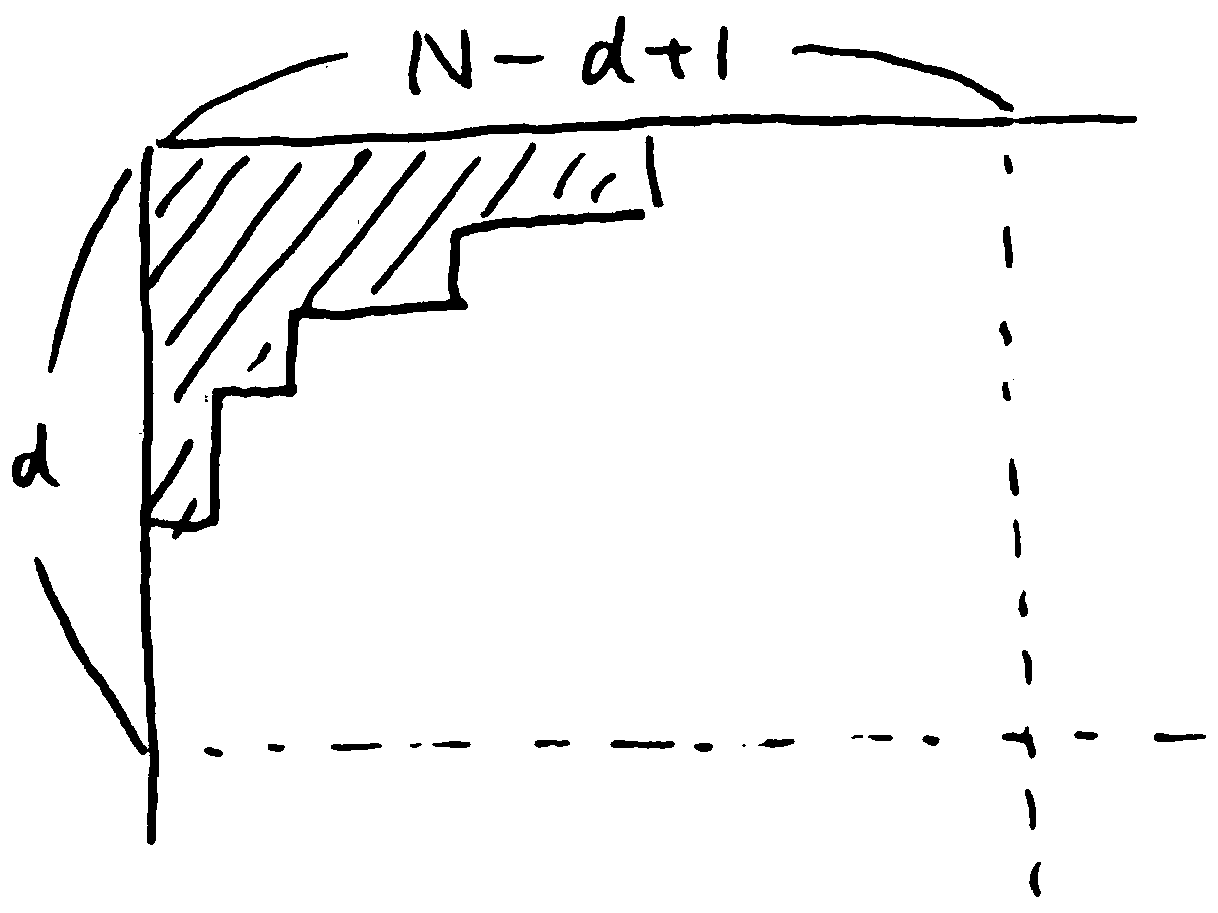
\includegraphics[width=0.62\linewidth]{fig_p87_a.png}
\end{center}
把 $W(f_1(0,t),\dots,f_d(0,t))$ 看作 $t$ 与 $\xi$ 的函数，称为 $\tau$ 函数。实际上，设对应的微分算子为 $W=W(t,V)=\partial^d+w_1\partial^{d-1}+w_2\partial^{d-2}+\cdots$，则存在某个 $P_i(\partial_t)=P_i\bigl(\frac{\partial}{\partial t_1},\dots,\frac{\partial}{\partial t_N}\bigr)$，使
\[
w_i=\frac{P_i(-\partial_t)\tau(t,\xi)}{\tau(t,\xi)}
\]
成立。（实际上 $P_i$ 是 complete monomial 的简单 modification。）也就是说，$W=W(t,V)$ 由 $\tau$ 函数表示。这里 $N$ 在形式上可以任意大，故 $\tau$ 可看作 $t_1,t_2,\dots$ 的函数。当然，若 $f_1,\dots,f_d\in\C\oplus\cdots\oplus\C x^N$，则 $\tau$ 实质上是 $t_1,\dots,t_N$ 的函数。若 $f_1,\dots,f_d\in\C[[x]]$，则 $\tau$ 是无穷多个变量 $t_1,t_2,\dots$ 的函数。

\subsection{佐藤方程与无穷维 Grassmann variety}

下面考虑 $W$ 所满足的微分方程。置 $z=t_1\partial+t_2\partial^2+\cdots$。由于 $W(t,V)$ 是作为消去 $\exp(z)f_1,\dots,\exp(z)f_d$ 的 monic $d$ 阶微分算子被刻画出来的，故
\[
W(t,V)\exp(z)f_i=0\qquad(i=1,\dots,d).
\]

\transnote{原书 p.81 此处印 $t_2\partial$，脱了平方；同一定义在 p.78 印作 $t_2\partial^2$，译文按 p.78 补出。}

\transnote{原书此句作「特徴付けられたのかから，」，在因果接续处有笔误（当作「特徴付けられたのだから，」），译文按因果关系处理。又，此处原书作 monomial $d$ 阶微分算子，与 p.78 的 monic 指同一意思，疑为笔误。}

两边对 $t_j$ 微分，得
\[
\Bigl(\frac{\partial W(t,V)}{\partial t_j}\exp(z)+W(t,V)\partial^j\exp(z)\Bigr)f_i=0\qquad(i=1,\dots,d)
\]
因此存在某个微分算子 $B_j(t,V)$，使
\[
(S_d)\qquad
\frac{\partial W(t,V)}{\partial t_j}+W(t,V)\partial^j=B_j(t,V)W(t,V)
\]

% ===== 原书 p.82 =====
成为如此。取 $W=\partial^d+w_1\partial^{d-1}+\cdots+w_d$ 时，这成为系数 $w_i=w_i(t_1,\dots,t_d)$ 关于 $t_i$ 的非线性偏微分方程。称之为佐藤方程，或称 KP 方程。综合以上可知：要得到佐藤方程的解，只须对 frame $\xi$，由 $\tau$ 函数 $\tau(t,\xi)$ 按 $(*)$ 式构造 $W$ 即可。对 $(S_d)$ 的解 $W$，$W\partial$ 是 $(S_{d+1})$ 的解。$(S_{d+1})$ 中满足 $w_{d+1}=0$ 者，正是这样得到的解全体。考虑这一点，则关于
\[
W=1+w_1\partial^{-1}+w_2\partial^{-2}+\cdots
\]
的方程
\[
(S)\qquad
\frac{\partial W(t,V)}{\partial t_j}+W(t,V)\partial^j=B_j(t,V)W(t,V)
\]
与 $w_{d+1}=w_{d+2}=\cdots=0$ 联立，把 $w_1,\dots,w_d$ 看作未知函数，所得的不是别的，正是 $(S_d)$。也就是说，令 $w_{d+1}=w_{d+2}=\cdots=0$，即可把 $(S_d)$ 的解看作 $(S)$ 的解。那么，具有无限多个 $w_1,w_2,\dots$ 的非平凡解应如何构造？取 $1,x,x^2/2!,\dots$ 作为 $\C[[x]]$ 的基，把其元素用列向量表示。把 $f_1,\dots,f_{d+1}\in\C[[x]]$ 并排所得的矩阵记作 $\xi$，考虑 $\xi$ 呈下述形状者。

\transnote{原书此页两处印「対いして」（「frame $\xi$ に対いして」「$(S_d)$ の解 $W$ に対いして」），多出的「い」为衍字（当作「対して」）；译文按原义译出。}
\[
\xi=(f_{d+1},\dots,f_1)=
\begin{pmatrix}
1 & 0 & \cdots & 0\\
a_{d+1,2} & 1 & \cdots & 0\\
a_{d+1,3} & a_{d,3} & \cdots & 0\\
 & \cdots & &
\end{pmatrix}
\]
再定义 $\xi'=(f'_d,\dots,f'_1)$，其中 $f'_1=\partial f_1,\dots,f'_d=\partial f_d$。也就是写成矩阵则
\[
\xi'=(f'_{d+1},\dots,f'_1)=
\begin{pmatrix}
1 & \cdots & 0\\
a_{d,3} & \cdots & 0\\
 & \cdots &
\end{pmatrix}
\]
成为如此。此时，$\tau(x,\xi')$ 关于 $S_Y$ 的系数 $\xi'_Y$ 与 $\tau(x,\xi)$ 关于 $S_Y$ 的系数 $\xi_Y$，在 Young tableau $Y$ 的深度不超过 $d$ 的范围内一致。回想 Young diagram 与 $0\le i_1<\cdots<i_{d+1}$ 的对应，即可明白。实际上，对 $0\le i_1<\cdots<i_{d+1}$ 相
% ===== 原书 p.83 =====
应的 Young diagram 深度不超过 $d$，也就是 $i_1=0$。考虑到第一行为 $(1,0,\dots,0)$，由 Pluecker 坐标定义中的 determinant 式即可立即看出。要妥善处理关于 $d$ 的相容性，把 frame $\xi$ 的行与列的原点按下图选取为好。
\begin{center}
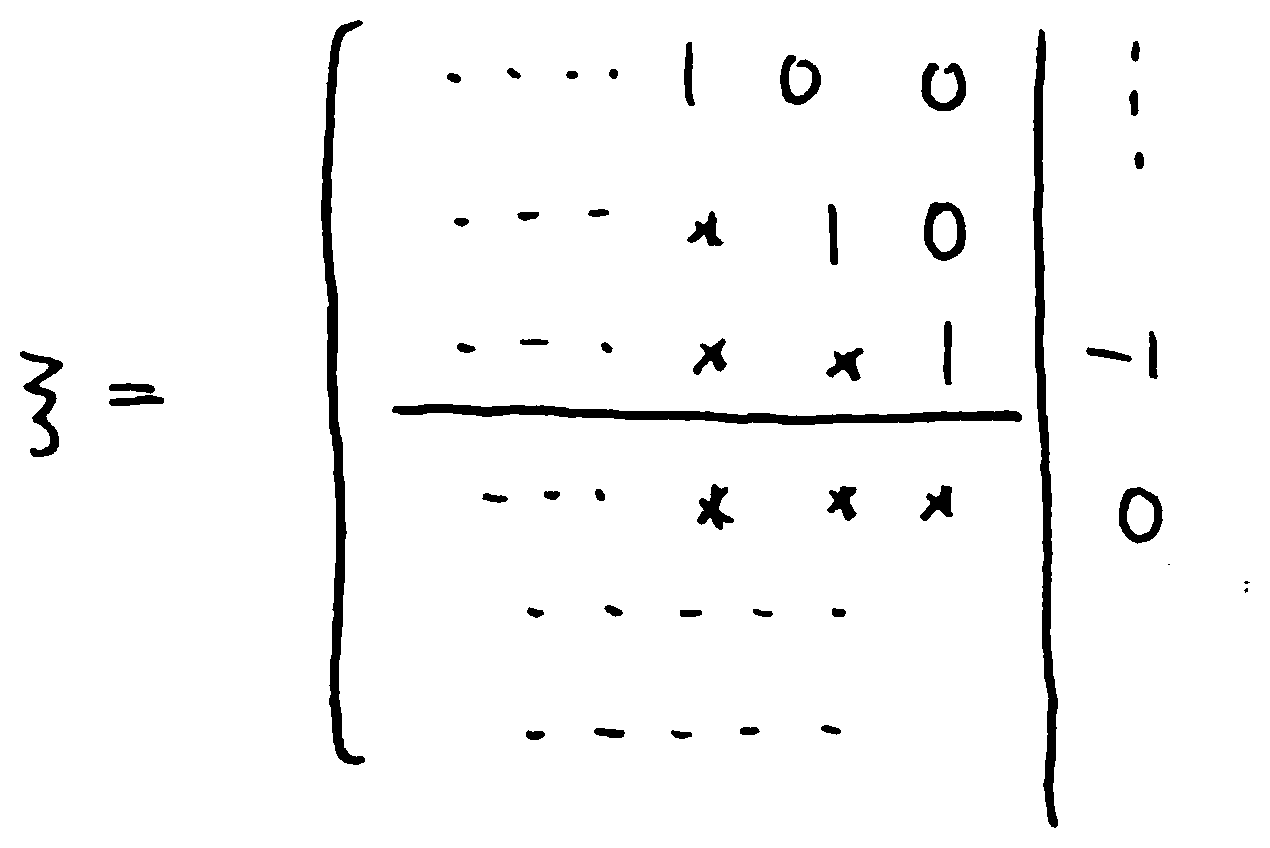
\includegraphics[width=0.55\linewidth]{fig_p89_a.png}
\end{center}
又，与 $Y$ 对应的 index 也只需考虑移动了原点的 Maya 图。Maya 图是指数列 $I=\{\cdots<i_{-3}<i_{-2}<i_{-1}\}$，且对充分大的 $m$ 有 $i_{-m}=-m$。它按下图用图形表示。
\[
\{i_{-4}<i_{-3}<i_{-2}<i_{-1}\}=\{-3,-1,2,4\}
\]
\begin{center}
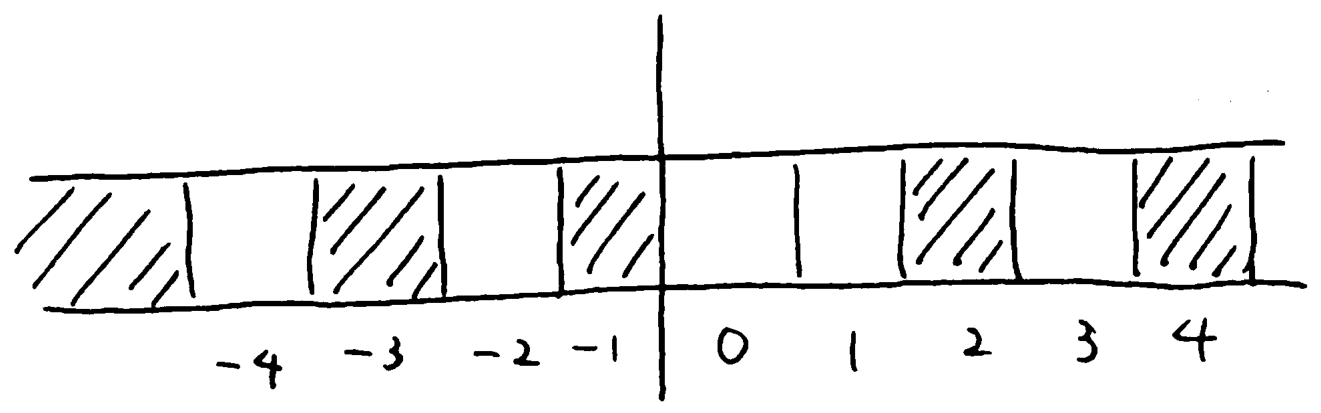
\includegraphics[width=0.78\linewidth]{fig_p89_b.png}
\end{center}
至此便可无碍地把 $\tau$ 函数看作带 frame 的无穷维 Grassmann variety 上的函数。作为 $\C[\partial]$-module，由 $x^n/n!\mapsto\partial^{-n-1}$ 这一对应，有 $\C[[x]]\simeq\C((\partial^{-1}))/\C[\partial]$。给出 $(*)$ 中 $\xi$ 的列向量，就是给出 $f\in\C((\partial^{-1}))$；而给出图 $(*)$ 之形的 $\xi$，等价于给出 $\C((\partial^{-1}))$ 的列 $f_i$ 且满足 $f_i\in\partial^i+\partial^{i-1}\C[[\partial^{-1}]]$（$i=1,2,\dots$）。这里要提醒的是：这样得到的 frame 属于 Grassmann variety 的某个开集，而并非全体。不过绝大多数都属于此，故以下只处理这样的 $\xi$。设 $\{\cdots<i_{-m}<\cdots<i_{-1}\}$ 为 Young diagram $Y$ 对应的 Maya 图，令 $f_i=\sum_j a_{ij}\partial^{-j}$，则 $\xi$ 的 Pluecker 坐
% ===== 原书 p.84 =====
% （本块末：此段起于 p.83，尚余两行在本块；§5.4 起属 c12）
标 $\xi_Y$ 用充分大的 $m$ 表示为
\[
\xi_Y=
\begin{pmatrix}
a_{mi_{-m}} & \cdots & a_{1i_{-m}}\\
\vdots & & \vdots\\
a_{mi_{-1}} & \cdots & a_{1i_{-1}}
\end{pmatrix}
\]
成为如此。此式与充分大的 $m$ 的取法无关。

\transnote{原书此处称「图 $(*)$」，但全书未见标为 $(*)$ 的图（p.82 的 $\xi$ 矩阵、p.83 的 $\xi$ 手绘图均无编号），此处照原文译出，所指待考。}

\transnote{原书正文作 $\xi'=(f'_d,\dots,f'_1)$，紧接的矩阵表示却作 $(f'_{d+1},\dots,f'_1)$，两处不一致，译文照原文排印。}
